\chapter{Successful architectures}


\section{Preliminaries}

\begin{description}
    \item[Stem layer] \marginnote{Stem layer}
        First convolutional layer of a CNN that aims to reduce the spatial size of the activations for memory and computational purposes
        but also to rapidly increase the receptive field.

    \item[Model parallelism] \marginnote{Model parallelism}
        Train a model by splitting its weights on multiple computational units, each receiving the same data.

    \item[Data parallelism] \marginnote{Data parallelism}
        Train a model by distributing the data on multiple computational units, each with a copy of the weights of the model.

    \item[Overlapping pooling] \marginnote{Overlapping pooling}
        Pooling layer with kernel size and stride chosen in such a way that
        some pixels at a step have also been considered at the previous one (e.g. $3 \times 3$ kernel with stride $2$).

    \item[Parameters computation] \marginnote{Parameters computation}
        \phantom{}
        \begin{description}
            \item[Input layer]
                Given an input image of shape $W_\text{in} \times H_\text{in} \times C_\text{in}$,
                the number of activations in the input layer is given by:
                \[ \texttt{\#activations} = W_\text{in} \cdot H_\text{in} \cdot C_\text{in} \]

                % As data is processed in batches of size $B$, the actual number of activations is:
                % \[ \texttt{\#activations\_batch} = B \cdot \texttt{\#activations} \]

            \item[Convolutional layer]
                Given:
                \begin{itemize}
                    \item An input of shape $W_\text{in} \times H_\text{in} \times C_\text{in}$,
                    \item A kernel of shape $W_\text{K} \times H_\text{K}$ with padding $P$ and stride $S$,
                    \item A desired number of output channels $C_\text{out}$,
                \end{itemize}
                the number of parameters of a convolutional layer (see \Cref{sec:conv_layer}) is given by:
                \[ \texttt{\#params} = \big( (W_\text{K} \cdot H_\text{K} \cdot C_\text{in}) + 1 \big) \cdot C_\text{out} \]

                The output shape (see \Cref{sec:conv_layer}) and the number of activations is given by:
                \[  
                    \begin{gathered}
                        \texttt{activ\_w} = \left\lfloor \frac{W_\text{in} - W_\text{K} + 2P}{S} \right\rfloor + 1 \hspace{2em}
                        \texttt{activ\_h} = \left\lfloor \frac{H_\text{in} - H_\text{K} + 2P}{S} \right\rfloor + 1 \\
                        \texttt{\#activations} = \texttt{activ\_w} \cdot \texttt{activ\_h} \cdot C_\text{out}
                    \end{gathered}    
                \]

                The number of FLOPs for a single example of the batch is given by:
                \[ \texttt{FLOPs} = \texttt{\#activations} \cdot (W_\text{K} \cdot H_\text{K} \cdot C_\text{in}) \cdot 2 \]

            \item[Pooling layer]
                Given:
                \begin{itemize}
                    \item An input of shape $W_\text{in} \times H_\text{in} \times C_\text{in}$,
                    \item A kernel of shape $W_\text{K} \times H_\text{K}$ with padding $P$ and stride $S$,
                \end{itemize}
                the number of activations in a pooling layer is computed as above with $C_\text{in} = C_\text{out}$:
                \[ \texttt{\#activations} = \texttt{activ\_w} \cdot \texttt{activ\_h} \cdot C_\text{in} \]

                The number of FLOPs for a single example of the batch is given by:
                \[ \texttt{FLOPs} = \texttt{\#activations} \cdot (W_\text{K} \cdot H_\text{K}) \]

            \item[Fully-connected layer]
                Given:
                \begin{itemize}
                    \item An activation of shape $C_\text{in}$,
                    \item The number of neurons $C_\text{out} = \texttt{\#activations}$,
                \end{itemize}
                the number of parameters of a fully-connected layer is:
                \[ \texttt{\#params} = (C_\text{in} \cdot C_\text{out}) + C_\text{out}\]

                The number of FLOPs for a single example of the batch is given by:
                \[ \texttt{FLOPs} = 2 \cdot C_\text{in} \cdot C_\text{out} \]

            \item[Memory usage]
                Given:
                \begin{itemize}
                    \item The batch size $B$, 
                    \item The activation size $\texttt{\#activations}$, 
                    \item The number of parameters $\texttt{\#params}$, 
                \end{itemize}
                to estimate the memory consumption, the following have to be taken into account:
                \begin{itemize}
                    \item To compute the gradient of the loss, every intermediate activation for every example in the batch has to be stored.
                    \item For every parameter, we have to store its value and the gradient of the loss w.r.t. it.
                    \item Optimizers with momentum need to store more values per parameter.
                \end{itemize}

                It is therefore hard to estimate memory requirements. 
                A rule of thumb estimates a lower bound as twice the activation size and 3-4 times the number of parameters.
                Assuming that $\texttt{float32}$ (4 bytes) are used, memory consumption is computed as:
                \[
                    \begin{gathered}
                        \texttt{memory\_activ\_bytes} = 2 \cdot (B \cdot \texttt{\#activations} \cdot 4) \\
                        \texttt{memory\_params\_bytes} = 3 \cdot (\texttt{\#params} \cdot 4)
                    \end{gathered}  
                \]
        \end{description}
\end{description}


\section{LeNet-5}
\marginnote{LeNet-5}

LeNet-5 is one of the first convolutional neural networks.
The network has the following properties:
\begin{itemize}
    \item At each layer, the number of channels increases and the spatial dimension decreases.
    \item Convolutions have the following characteristics: $5 \times 5$ kernels, no padding and average pooling for down-sampling.
    \item \texttt{Sigmoid} and \texttt{tanh} activation functions are used, with carefully selected amplitudes (i.e. they are scaled).
    \item The last layers are fully connected with a radial basis function as the output activation.
    \item There are no residual connections and normalization layers.
\end{itemize}

\begin{figure}[H]
    \centering
    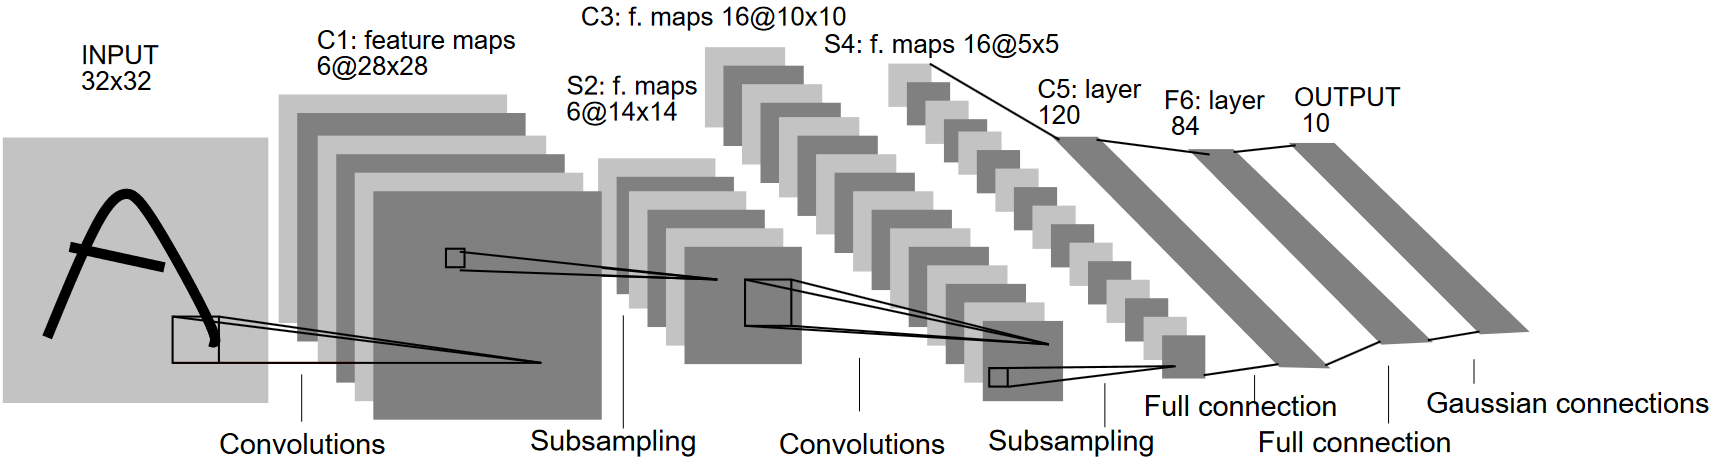
\includegraphics[width=0.8\linewidth]{./img/lenet5.png}
\end{figure}



\section{AlexNet}
\marginnote{AlexNet}

AlexNet is the first CNN that broke the stagnation of the field.


\subsection{Architecture}

AlexNet is composed of:
\begin{itemize}
    \item 5 convolutional layers (convolution + \texttt{ReLU}, sometimes with max-pooling).
    \item 3 feed-forward layers.
\end{itemize}

\begin{figure}[H]
    \centering
    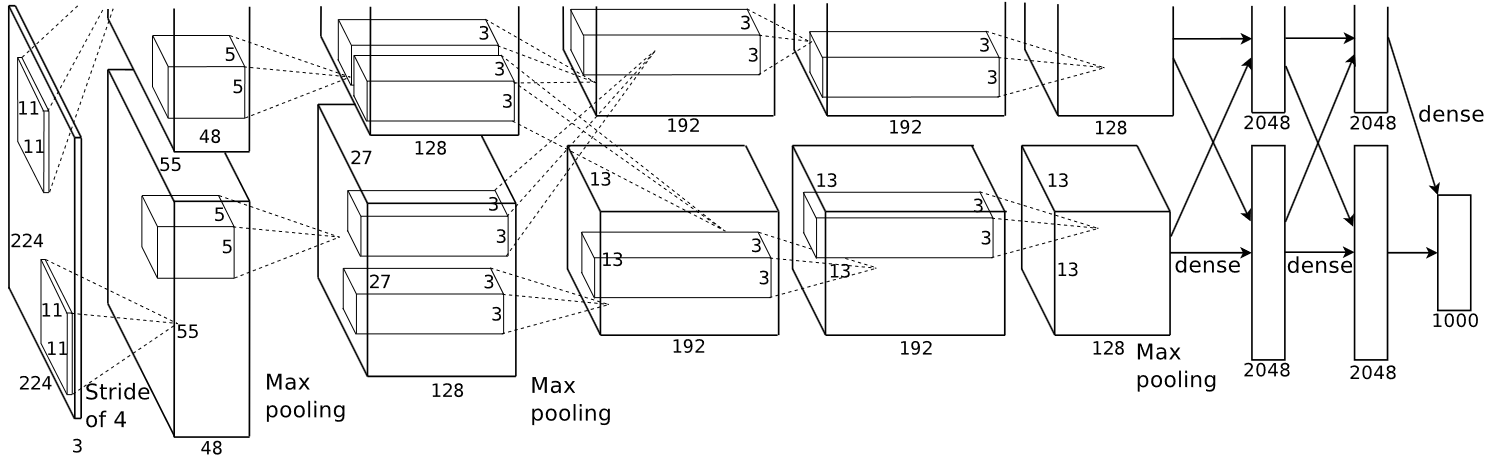
\includegraphics[width=0.8\linewidth]{./img/alexnet.png}
\end{figure}


\subsection{Training}

The network is trained on ImageNet 1k (for the ILSVRC 2012) with a batch size of 128.
Due to GPU memory limitations, training was split into two parallel lines on two GPUs (model parallelism).

\begin{description}
    \item[Grouped convolution] \marginnote{Grouped convolution}
        A convolution is split into two sets of weights, each trained independently on a computational line.
        At some steps (e.g. \texttt{conv3}), the two GPUs are allowed to communicate.
        In this case, the result of the operation can be virtually seen as if it was done by a single computational unit (i.e. the operation is done on the full set of weights).
\end{description}

\begin{remark}
    At the time, training took 5-6 days on two Nvidia GTX 580.
\end{remark}


\subsection{Properties}

AlexNet has the following trends:
\begin{itemize}
    \item The first convolutional layer is a stem layer.
    \item The majority of the parameters are in the fully connected layers (even though they have to process an activation of 4096 elements).
    \item The largest memory consumption for activations is at the first convolutional layer.
    \item The largest amount of FLOPs is required by the convolutional layers.
    \item The total number of parameters and activations at training time are relatively comparable.
    \item $2.2$ GFLOPs are required to process an image at training time.
\end{itemize}

\begin{table}[H]
    \centering
    \caption{Parameters of AlexNet (batch size of 128)}
    \small
    \begin{tabular}{cccccccccccc}
        \toprule
        \multirow{2}[20]{*}{\textbf{Layer}} 
            & \multicolumn{4}{c}{\textbf{Convolution}} 
            & \multicolumn{3}{c}{\textbf{Single activation}} 
            & \multirow{2}[20]{*}{\texttt{\#params}} 
            & \multicolumn{3}{c}{\textbf{Batch requirements}} \\
        \cmidrule(lr){2-5} \cmidrule(lr){6-8} \cmidrule(lr){10-12}
            & \rot{\textbf{Channels}} & \rot{\textbf{H/W}} & \rot{\textbf{Stride}} & \rot{\textbf{Padding}} 
            & \rot{\textbf{H/W}} & \rot{\textbf{Channels}} & \rot{\texttt{\#activ.}} 
            & 
            & \rot{\textbf{MFLOPs}} & \rot{\textbf{Activ. mem.}} & \rot{\textbf{Params mem.}} \\
        \midrule
        \texttt{input}      &             &             &             &         & \num{227}   & \num{3}     & \num{154587}    & \num{0}         & --              & \num{75.5} MB  & \num{0.0}      \\
        \texttt{conv1}      & \num{96}    & \num{11}    & \num{4}     & \num{0} & \num{55}    & \num{96}    & \num{290400}    & \num{35} K      & \num{26986.3}   & \num{283.6} MB & \num{0.4} MB   \\
        \texttt{pool1}      & \num{1}     & \num{3}     & \num{2}     & \num{0} & \num{27}    & \num{96}    & \num{69984}     & \num{0}         & \num{80.6}      & \num{68.3} MB  & \num{0.0}      \\
        \texttt{conv2}      & \num{256}   & \num{5}     & \num{1}     & \num{2} & \num{27}    & \num{256}   & \num{186624}    & \num{615} K     & \num{114661.8}  & \num{182.3} MB & \num{7.0} MB   \\
        \texttt{pool2}      & \num{1}     & \num{3}     & \num{2}     & \num{0} & \num{13}    & \num{256}   & \num{43264}     & \num{0}         & \num{49.8}      & \num{42.3} MB  & \num{0.0}      \\
        \texttt{conv3}      & \num{384}   & \num{3}     & \num{1}     & \num{1} & \num{13}    & \num{384}   & \num{64896}     & \num{885} K     & \num{38277.2}   & \num{63.4} MB  & \num{10.1} MB  \\
        \texttt{conv4}      & \num{384}   & \num{3}     & \num{1}     & \num{1} & \num{13}    & \num{384}   & \num{64896}     & \num{1327} K    & \num{57415.8}   & \num{63.4} MB  & \num{15.2} MB  \\
        \texttt{conv5}      & \num{256}   & \num{3}     & \num{1}     & \num{1} & \num{13}    & \num{256}   & \num{43264}     & \num{885} K     & \num{38277.2}   & \num{42.3} MB  & \num{10.1} MB  \\
        \texttt{pool3}      & \num{1}     & \num{3}     & \num{2}     & \num{0} & \num{6}     & \num{256}   & \num{9216}      & \num{0}         & \num{10.6}      & \num{9.0} MB   & \num{0.0}      \\
        \texttt{flatten}    & \num{0}     & \num{0}     & \num{0}     & \num{0} & \num{1}     & \num{9216}  & \num{9216}      & \num{0}         & \num{0.0}       & \num{0.0}      & \num{0.0}      \\
        \texttt{fc6}        & \num{4096}  & \num{1}     & \num{1}     & \num{0} & \num{1}     & \num{4096}  & \num{4096}      & \num{37758} K   & \num{9663.7}    & \num{4.0} MB   & \num{432.0} MB \\
        \texttt{fc7}        & \num{4096}  & \num{1}     & \num{1}     & \num{0} & \num{1}     & \num{4096}  & \num{4096}      & \num{16781} K   & \num{4295.0}    & \num{4.0} MB   & \num{192.0} MB \\
        \texttt{fc8}        & \num{1000}  & \num{1}     & \num{1}     & \num{0} & \num{1}     & \num{1000}  & \num{1000}      & \num{4097} K    & \num{1048.6}    & \num{1.0} MB   & \num{46.9} MB  \\
        \midrule
        &&&&&&& \textbf{Total} & \num{62378} K & \num{290851} & \num{1.406} MB & \num{714} MB \\
        \bottomrule
    \end{tabular}
\end{table}

